% !TEX root = ../../main.tex

\section{Model and Training Strategy}\label{sec:model}
In this section, we first define \maskname masks in Sec.~\ref{sec:self_masks}.
Then, in Sec. \ref{sec:encoding_masks}, we present our first main contribution, a model trained end-to-end to predict encoded \maskname masks, one for each pixel of the input image. 
% Finally, in Sec. \ref{sec:multiscale_patches}, we show how we predicted \maskname masks at different scales.

\subsection{Local Central Instance Masks}\label{sec:self_masks}
The method presented here proposes to distinguish between different object instances based on instance-aware pixel-pair affinities in the interval $[0,1]$, which specify whether or not two pixels belong to the same instance or not.
Given a pixel of the input image with coordinates $\coord{u}= (u_x, u_y)$, a set of affinities to neighboring pixels within a $K\times K$ window is learned, where $K$ is an odd number. 
We define the $K\times K$-neighborhood of a pixel as: 
$\mathcal{N}_{K\times K} \equiv \mathcal{N}_{K} \times \mathcal{N}_{K}$, where $\mathcal{N}_{K} \equiv \left\{-\frac{K-1}{2}, \ldots, \frac{K-1}{2}\right\}$ and represent the affinities relative to pixel $\coord{u}$ as a \maskname mask $\mathcal{M}_{\coord{u}}: \mathcal{N}_{K\times K} \rightarrow [0,1]$.

% In total, if the input image has $H\times W$ pixels, we predict $K^2 \times H \times W$ affinities. 
We represent the associated training targets as binary ground-truth masks $\hat{\mathcal{M}}_{\coord{u}}: \mathcal{N}_{K\times K} \rightarrow \{0,1\}$, which can be derived from a ground-truth instance label image $\hat{L}: H\times W \rightarrow \mathbb{N}$ with dimension $H\times W$:
\begin{equation}\label{eq:target_masks}
\forall\, \coord{u}\in H\times W, \quad \forall\, \coord{n}\in \mathcal{N}_{K\times K} \qquad \hat{\mathcal{M}}_{\coord{u}}(\coord{n}) = 
\begin{cases}
1, \quad &\text{if } \hat{L}(\coord{u}) = \hat{L}(\coord{u}+\coord{n}) \\
0, \quad & \text{otherwise}.
\end{cases}
\end{equation}
We actually use similar definitions in 3D, but use 2D notation here for simplicity.


\begin{figure}[t]
\centering
\begin{minipage}[t]{0.36\textwidth}
        \centering
        % \includegraphics[width=0.4\textwidth,trim=0.25in 0.25in 0.68in 0.36in,clip]{./figures/LSIMasks/SSBM_experiments.pdf} % 0.45
        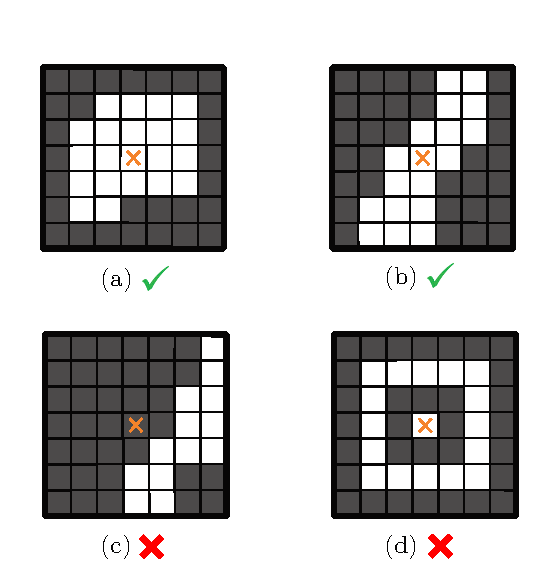
\includegraphics[width=0.99\textwidth]{./figures/LSIMasks/valid_masks.pdf} % 0.45
        \captionof{figure}{Examples of expected (\textbf{a-b}) and not expected (\textbf{c-d}) binary 2D \maskname masks. }
    \label{fig:valid_masks}
\end{minipage}\hfill
\begin{minipage}[t]{0.58\textwidth}
\centering
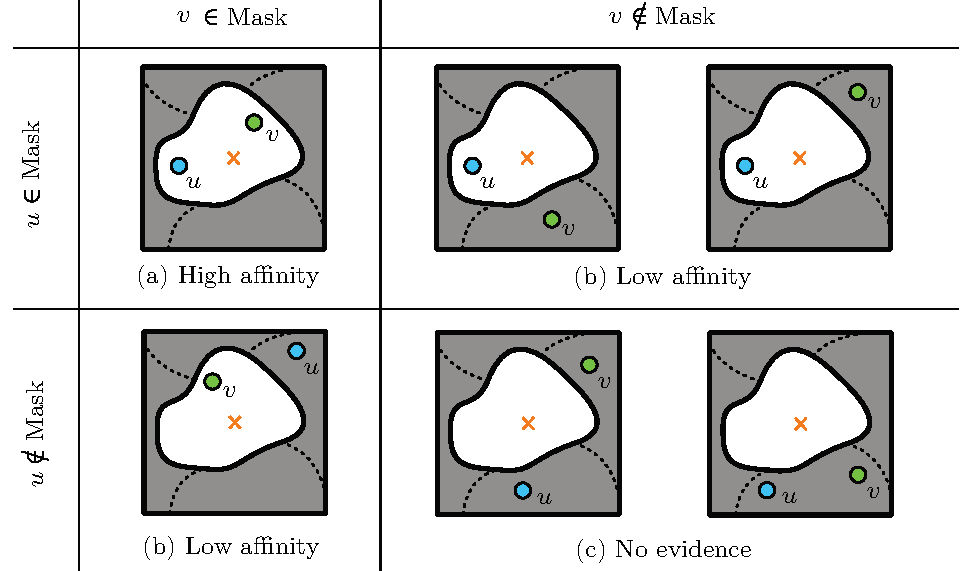
\includegraphics[width=0.99\textwidth]{./figures/LSIMasks/mask_cases_new.pdf} % 0.45
        \captionof{figure}{Computing instance-aware affinity between pixels $u$ and $v$ from instance masks associated to the central pixel in the patch (orange cross). 
        % Dashed lines represent ground-truth boundaries separating neighboring segments. 
        % We distinguish three cases: \textbf{(a)} when both pixels are part of the mask, a high affinity between the pixels is predicted; \textbf{(b)} when only one of them is part of the mask, we predict a low affinity; \textbf{(c)} when both pixels are not part of the mask, nothing can be said about their affinity.
        }
    \label{fig:mask_cases}
\end{minipage}
\end{figure}

\subsection{Training Encoded Central Instance Masks End-To-End}\label{sec:encoding_masks}
% In this section, we briefly review the strong baseline model used in our comparison experiments that has been widely used in instance segmentation  (see \emph{\sparseBr branch} in Fig. \ref{fig:main_figure}a).
In several related work approaches \cite{liu2018affinity,Gao_2019_ICCV,lee2017superhuman,wolf2018mutex,bailoni2019generalized}, affinities between pairs of pixels are predicted for a predefined sparse stencil representing a set of $N$ short- and long-range neighborhood relations for each pixel  ($N=8$ \emph{\sparseBr branch} of Fig. \ref{fig:main_figure}a). The $N$ output feature maps  are then trained with a binary classification loss. 
% In other words, we do not predict one full \maskname mask for each pixel of the input image, but only a predefined pattern of $N$ out of $K\times K$ pixels of each \maskname mask. 
% As shown in the \emph{\sparseBr branch} of Fig. \ref{fig:main_figure}a, the backbone model is trained to output $N$ feature maps, each representing a different neighborhood relation. We then define a dense channel-wise S\o rensen-Dice loss for every pixel \cite{wolf2018mutex,dice1945measures,sorensen1948method}.
% As compared to L2 or binary cross-entropy, this loss is more robust against class imbalance.
% prediction and / or target sparsity, a desirable quality for our application in neuron segmentation, since transitions between neuron instances occupy very few pixels in a three-dimensional volume.


On paper, this training method can be easily generalized to output a feature map of size $K^2 \times H \times W$ and thus predict a full $K\times K$ \maskname mask for each pixel of the input image (see \emph{\denseBr branch} in Fig. \ref{fig:main_figure}b).
Nevertheless, in practice, this model has prohibitively large memory requirements for meaningful values of $K$, precluding application to 3D data of interest here.

However, among the $2^{K\cdot K}$ conceivable binary masks $\hat{\mathcal{M}}_{\coord{u}}: \mathcal{N}_{K^2} \rightarrow \{0,1\}$, in practice only a tiny fraction corresponds to meaningful instance masks (see some examples in Fig. \ref{fig:valid_masks}). 
This suggests that it is possible to find a compact representation that spans the manifold of expected instance shapes.

As our first main contribution, we test this assumption by training a model end-to-end to predict, for each pixel $\coord{u}\in H\times W$ of the input image, a latent vector $z_{\coord{u}}\in \mathbb{R}^Q$ encoding the $K \times K$ \maskname mask $\mathcal{M}_{\coord{u}}$ centered at pixel $\coord{u}$ (see \emph{\encBr branch} in Fig. \ref{fig:main_figure}c). 
The backbone model is first trained to output a more compact $Q\times H\times W$ feature map and
% as compared to $K^2 \times H \times W$. 
then a tiny convolutional decoder network is applied to each pixel of the feature map to decode masks.
During training, decoding one mask for each pixel in the image would be too memory consuming. Thus, we randomly sample $R$ pixels with coordinates $\coord{u}_1, \ldots, \coord{u}_R$ and only decode the associated masks $\mathcal{M}_{\coord{u}_1}, \ldots, \mathcal{M}_{\coord{u}_R}$. 
Given the ground-truth \maskname masks $\hat{\mathcal{M}}_{\coord{u}_i}$ defined in Eq. \ref{eq:target_masks}, the training loss is then defined according to the S\o rensen-Dice coefficient formulated for fuzzy set membership values, similarly to what was done in \cite{wolf2018mutex}.
% \begin{equation}
% \mathcal{J}_{\mathrm{MaskLoss}} = - \frac{\sum_{i=1}^R \sum_{\coord{n} \in \mathcal{N}_{K\times K}} \big(1-\mathcal{M}_{\coord{u}_i}(\coord{n})\big)\cdot \big(1-\hat{\mathcal{M}}_{\coord{u}_i}(\coord{n})\big)}{\sum_{i=1}^R \sum_{\coord{n}\in \mathcal{N}_{K\times K}} \Big( \big(1-\mathcal{M}_{\coord{u}_i}(\coord{n})\big)^2 + \big(1-\hat{\mathcal{M}}_{\coord{u}_i}(\coord{n})\big)^2 \Big)}.
% \end{equation} 
Ground-truth labels are not always pixel-precise and it is often impossible to estimate the correct label for pixels that are close to a ground-truth label transition. Thus, in order to avoid noise during training, we predict completely empty masks for pixels that are less than two pixels away from a label transition, so that the model is trained to predict single-pixel clusters along the ground-truth boundaries. In our experiments, this approach performed better than masking the training loss along the boundaries.


\subsection{Predicting Multi-Scale Central Instance Masks}\label{sec:multiscale_patches}
Previous related work \cite{lee2017superhuman,liu2018affinity,Gao_2019_ICCV} shows that predicting long-range affinities between distant pixels improves accuracy as compared to predicting only short-range ones. However, predicting large \maskname masks would translate to a bigger model that, on 3D data, would have to be trained on a small 3D input field of view.
This, in practice, usually decreases accuracy because of the reduced 3D context available to the network.
% whose size is an important hyper-parameter in neuron segmentation since the correct detection of mitochondria and other organelles strongly depends on how much surrounding 3D context is provided during training.
Thus, we instead predict multiple \maskname masks of the same window size $7 \times 7 \times 5$ but at different resolutions, so that the lower the resolution the larger the size of the associated patch in the input image. 
% Note that the size of \maskname masks in this work is kept fixed only for simplicity reasons.
These multiple masks at different resolutions are predicted by adding several \emph{\encBr branches} along the hierarchy of the decoder in the backbone model, which in our case is a 3D U-Net \cite{ronneberger2015u,cciccek20163d} (see Fig.~\ref{fig:model_architecture}). 
In this way, the encoded \maskname masks at higher and lower resolutions can be effectively learned at different levels in the feature pyramid of the U-Net.



